% ycb1-fig-overview-nervious-system. Labels from notes block ycb1-hl-human-body-introduction,
% "Nervous system divisions" and "Nervous" bullets (checked).
\documentclass[border=6pt]{standalone}
% Shared preamble for the YCB1 line diagrams (standalone TikZ, XeTeX). Black and white only; labels come from
% the checked notes block named in each diagram file. Build: make_figures.bat in this folder.
\usepackage{fontspec}
\setmainfont{Segoe UI}
\usepackage{tikz}
\usetikzlibrary{arrows.meta,positioning,shapes.geometric,calc,decorations.pathreplacing}
\hyphenpenalty=10000 \exhyphenpenalty=10000 % no hyphenated labels
\tikzset{
  box/.style={draw, rounded corners=2pt, align=center, inner sep=4pt, font=\small, minimum height=1.6em},
  head/.style={box, font=\small\bfseries},
  note/.style={align=center, font=\footnotesize},
  link/.style={-{Stealth[length=2mm]}, thin},
}

\begin{document}
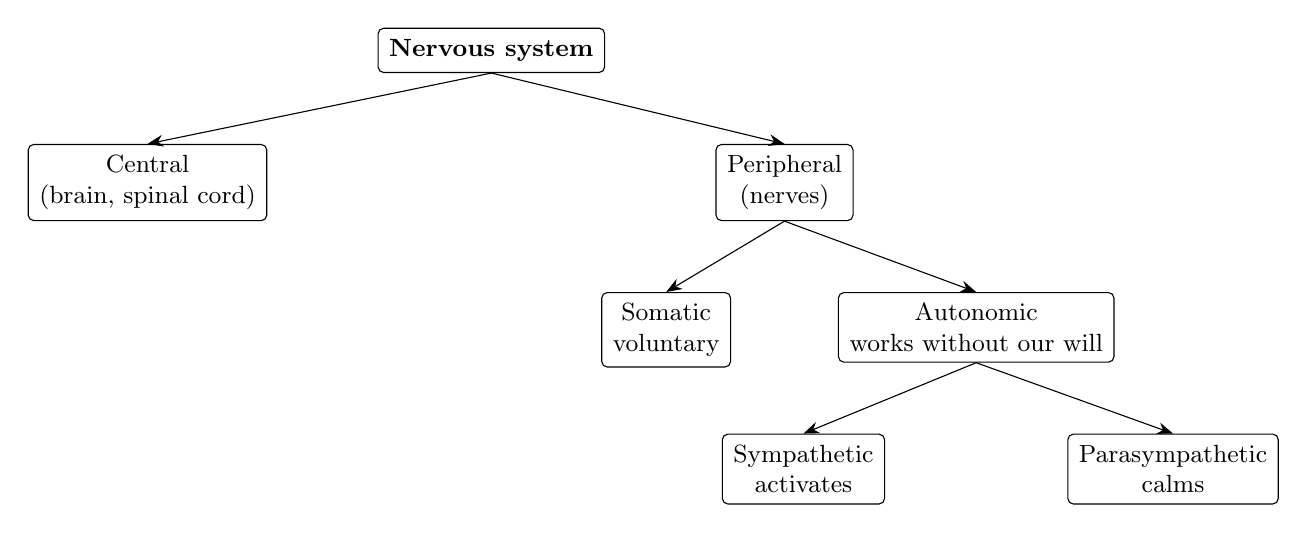
\begin{tikzpicture}[level distance=13mm]
\node[head] (ns) {Nervous system};
\node[box, below left=9mm and 14mm of ns] (cns) {Central\\(brain, spinal cord)};
\node[box, below right=9mm and 14mm of ns] (pns) {Peripheral\\(nerves)};
\node[box, below left=9mm and -2mm of pns] (som) {Somatic\\voluntary};
\node[box, below right=9mm and -2mm of pns] (aut) {Autonomic\\works without our will};
\node[box, below left=9mm and -6mm of aut] (sym) {Sympathetic\\activates};
\node[box, below right=9mm and -6mm of aut] (par) {Parasympathetic\\calms};
\foreach \a/\b in {ns/cns, ns/pns, pns/som, pns/aut, aut/sym, aut/par}
  \draw[link] (\a.south) -- (\b.north);
\end{tikzpicture}
\end{document}
